\section{Описание контейнера}
Бинарное (двоичное) дерево (binary tree) - это упорядоченное дерево, каждая вершина которого имеет не более двух поддеревьев, причем для каждого узла выполняется правило: в левом поддереве содержатся только ключи, имеющие значения, меньшие, чем значение данного узла, а в правом поддереве содержатся только ключи, имеющие значения, большие, чем значение данного узла.

Бинарное дерево является рекурсивной структурой, поскольку каждое его поддерево само является бинарным деревом и, следовательно, каждый его узел в свою очередь является корнем дерева.

Узел дерева, не имеющий потомков, называется листом.

Схематичное изображение бинарного дерева:
\begin{center}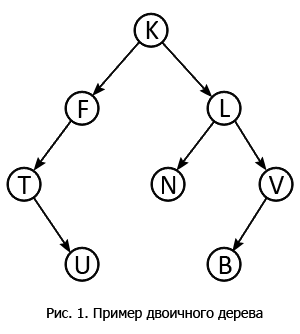
\includegraphics{1.png}\end{center}

Организация данных с помощью бинарных деревьев часто позволяет значительно сократить время поиска нужного элемента. Поиск элемента в линейных структурах данных обычно осуществляется путем последовательного перебора всех элементов, присутствующих в данной структуре. Поиск по дереву не требует перебора всех элементов, поэтому занимает значительно меньше времени. Максимальное число шагов при поиске по дереву равно высоте данного дерева, т.е. количеству уровней в иерархической структуре дерева.

Бинарное дерево является рекурсивной структурой, поскольку каждое его поддерево само является бинарным деревом и, следовательно, каждый его узел в свою очередь является корнем дерева.

При работе с деревьями обычно используются рекурсивные алгоритмы. Использование рекурсивных функций менее эффективно, поскольку многократный вызов функции расходует системные ресурсы. Тем не менее, использование рекурсивных функций является оправданным, поскольку нерекурсивные функции для работы с деревьями гораздо сложнее и для написания, и для восприятия кода программы.

Основные операции в бинарном дереве:

\begin{itemize}
\item обход дерева;
\item добавление элемента;
\item удаление элемента;
\item поиск элемента;
\end{itemize}

\begin{center}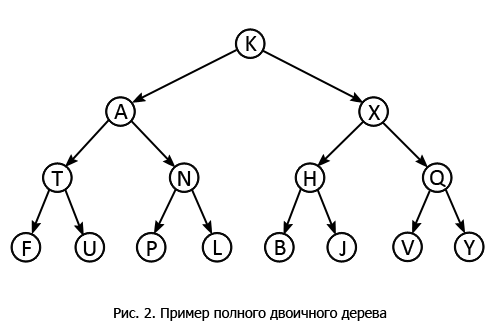
\includegraphics{2.png}\end{center}

Операция, при которой вершины дерева поочередно просматриваются и каждая только один раз называется {\bf обходом дерева}. Выделяют четыре основных метода обхода:

\begin{itemize}
\item обход в ширину;
\item прямой обход;
\item обратный обход;
\item симметричный обход;
\end{itemize}

{\bf Обход в ширину} – это поуровневая обработка узлов слева на право. Работа этого метода заключается в просмотре всех вершин, начиная с n-ого уровня и некоторой вершины.

Возьмем нулевой уровень за начальный (рис. 2), и, начиная с вершины K, будем методом обхода в ширину поочередно двигаться вниз, просматривая при этом вершины в следующем порядке: K A X T N H Q F U P L B J V Y.

{\bf Обход в прямом порядке} вначале предполагает обработку предков, а потом их потомков, то есть сначала посещается вершина дерева, далее левое и правое поддеревья, именно в описанном порядке. Для нашего дерева последовательность прямого обхода такая: K A T F U N P L X H B J Q V Y.

{\bf Обход в обратном порядке} противоположен прямому обходу. Первыми осматриваются потомки, а уже затем предки, иначе говоря, первоначально обращение идет к элементам нижних уровней левого поддерева, потом то же самое с элементами правого, и в конце осматривается корень. Обратный обход дерева с рисунка 2: F U T P L N A B J H V Y Q X K.

{\bf Обход в симметричном порядке} заключается в посещении левого узла, перехода в корень, и оттуда в правый узел. Все для того же дерева узлы будут осмотрены в следующем порядке: F T U A P N L K B H J X V Q Y.

Узел бинарного дерева можно описать следующим образом:
\begin{lstlisting}[language=C++, caption="Описание узла бинарного дерева на С++"]
struct BTree
{
	T data;
	BTree* left;
	BTree* right;
};
\end{lstlisting}

Где Т - тип данных хранимых внутри узла, а left и right - указатели на левое и правое дочерное поддерево узла.

Как в случае со списком, программа должна хранить указатель на первый элемент дерева, его вершину, который ещё называют {\bf корнем дерева} (Root). В начале работы программы дерево пусто и корневой элемент может быть определён как {\it BTree* Root = NULL;}.

